\section{绘图}
\label{sec:display}

SAC中有四个常用的绘图命令,分别是~\nameref{cmd:plot}、\nameref{cmd:plot1}、
\nameref{cmd:plot2}、\nameref{cmd:plotpk}。这一节通过plot和plot1命令简单介绍一下SAC的绘图功能,其他的命令及更多的绘图功能将在``~\nameref{chap:sac-graphics}~''中说明。

\subsection{plot}
\label{subsec:plot}
plot命令会在单个图形窗口中显示单个波形。
\begin{SACCode}
SAC> r cdv.[nez]
SAC> p
Waiting
Waiting
SAC>
\end{SACCode}

鉴于在SAC绘图中有很多中文意思类似的名词,这里似乎有必要定义一下``窗口''。图
\ref{fig:plot}~展示了一个SAC窗口。同很多其它软件界面类似,这个窗口在左上角显示
图标,右上角显示``最小化''、``最大化''、``还原''和``关闭''按钮。

左上角的``Graphics Window: 1''指明了当前绘图窗口的编号为``1''。SAC中一共可以同时
使用10个类似的窗口。

窗口的中间部分为真正的绘图区,以后的图将只显示绘图区而不显示整个窗口。

\begin{figure}[H]
\centering
\includegraphics[width=0.95\textwidth]{plot}
\caption{绘图窗口}
\label{fig:plot}
\end{figure}

将三个波形数据读入内存,使用plot时,焦点位于绘图窗口,且绘图窗口上只显示
第一个波形,终端中出现``Waiting''字样;将焦点切换\footnote{Linux下的快捷键是Alt+Tab。}回终端,
敲击回车键,绘图窗口中显示第二个波形,终端中出现第二个``Waiting''字样,
焦点位于终端中;再次敲击回车键,窗口中显示第三个波形,焦点位于终端,
由于已经没有更多的波形需要显示,此时终端中显示SAC提示符。

如果内存中还有波形在``Waiting'',而你想要退出plot,不想要再继续查看后面的波形,
可以在终端中键入``kill''(简写为k),以直接退出plot,如下例:
\begin{SACCode}
SAC> r cdv.[nez]
SAC> p
Waitingk
SAC>
\end{SACCode}

也许你已经发现,即使plot结束或者中途退出plot,绘图窗口依然没有被关闭,而且即便
点击窗口的``关闭''按钮,窗口依然无法关闭。
\begin{SACCode}
SAC> r cdv.[nez]
SAC> begindevices xwindows      // 启动图像设备xwindows,简写为bd x
SAC> p
Waiting
Waiting
SAC> enddevices xwindows        // 关闭图像设备xwindows,简写为ed x
\end{SACCode}
严格地说,SAC绘图的流程应该是:启动图像设备(xwindows或者sgf)$\rightarrow$绘图$\rightarrow$关闭图像设备。
这样稍显繁琐,SAC将这一流程进行了简化,在每次绘图前偷偷启动了SAC默认的图像设备xwindows,
也就是上面所说的窗口,而关闭图像设备这一步需要用户自己完成,当然,在退出SAC时,SAC
也会自动关闭图像设备。

\subsection{plot1}
plot1命令会在一个窗口中显示多个波形。这些波形共用一个X轴,但拥有单独的Y轴。
\begin{SACCode}
SAC> r cdv.?
cdv.e cdv.n cdv.z
SAC> p1
\end{SACCode}
执行plot1命令后,焦点位于图形窗口,显示如图~\ref{fig:plot1}。
\begin{figure}[H]
\centering
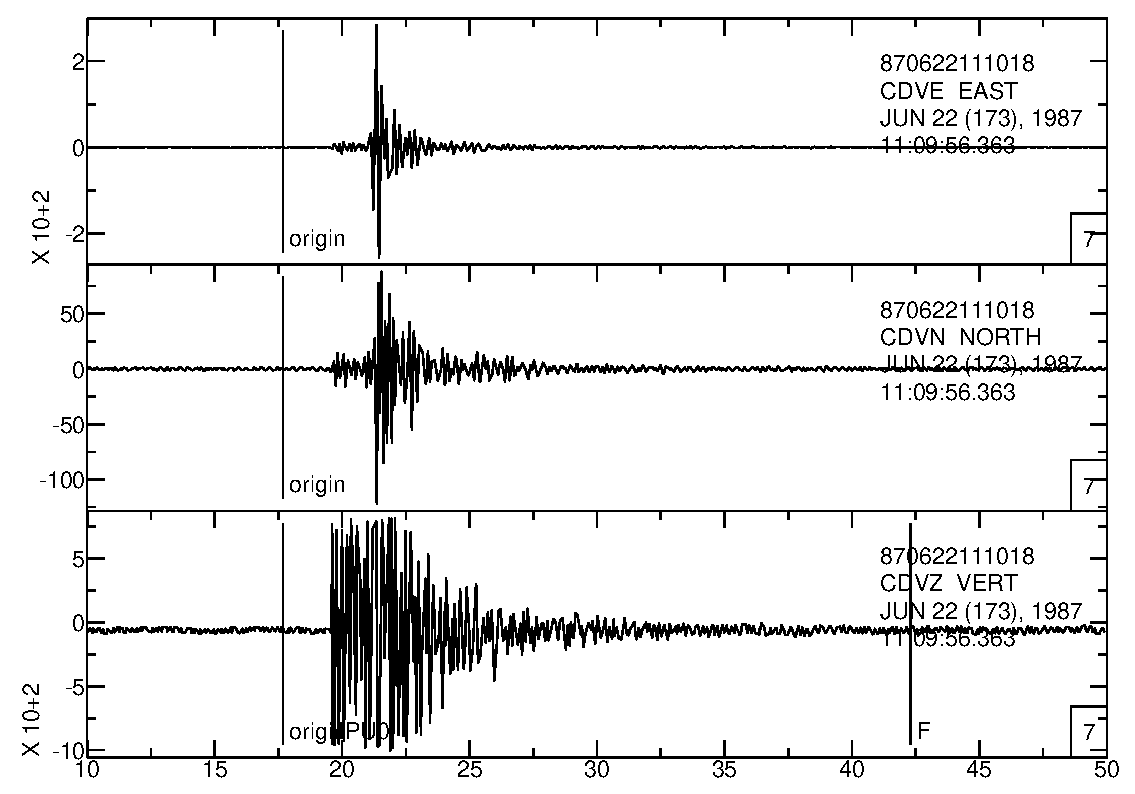
\includegraphics[width=0.85\textwidth]{plot1}
\caption{plot1绘图效果}
\label{fig:plot1}
\end{figure}
